\chapter{Apparatus}
\label{Chap_Apparatus}

% epigraph
\setlength{\unitlength}{1pt}
\setlength{\epigraphwidth}{10cm}
\epigraph{工欲善其事,必先利其器。\\ A craftsman must sharpen his tools to do his job.}{--- Confucius\\ \textit{The Analects}}

% guide
In this chapter, we decribe the Na-Rb machien and upgrades we done for our droplet experiment. As most of the machine has been described by previous thesis(add ref here), we only shortly make a summary of them to make the completenees of this chapter. Then, we turn to the image system upgrades, including the optical part and machenical part. Then, we introduce the high field insitu image method for 提取 sampele's density profile reliable. Finally, we discuss several improvement such as fast coil for fast control magnetic field and improvement of the coil antenna.

\section{Overview: Na-Rb machine I}
% aim
A repeatable machien for producing stable sample with satable number, density temperature and so on, is imprtant to carry out the following experiment. So, even this Na-Rb machien has been run for longer than 8 years, there still many aspect need to improve to make the sample 状态  more stable. Besides stablity, more atom is another 追求, for many experiment, as more atom number is better for showing the many body aspect properties. So, to improve our machine to achieve more atom number is better. We persue more and cooler sample condition as possible. 

% How
Our machien start from Na and Rb dispensor. We fire our Rb dispensor every day with a relatively low  current and Na fire only once a month. The atom typically absorbed by the 腔壁 of vacuum chamber. So, we use LIAD to disabsorped the atom to the vacuum at the beginning of each shot. With the atom gradually acuumulated in 30s, our MOT capture increasing number of atoms. To avoid Rb occupating Na MOT possitin, we use a resonance light to push 一点 of the Rb MOT aside. That is out double MOT which typically can capture $10^{10}$ Rb and $10^{9}$ Na(number need check). Then, to increase its density, we apply a CMOT process to increase its density and PSD by incresing the detuning the MOT laser and increase the gradient of magnetic field. (actually, we increase no QT) Then, a molasses process to decrease the temperature of the sample then we can load the sample to QT. The QT is with gradient around 160 G/cm which is a quite deep trap as a conservation trap for capture enough number of atoms. Then, we do the evaporation cooling for Rb which using a MW to pump Rb1,-1, to 2,0 to remove the high tempreture Rb away from the trap to decrease the sampel temperature. 


\subsection{Production of Na-Rb Bose-Einstein condensate mixtures}
\subsection{Production of Na-Rb Feshbach molecules}

\section{Image system upgrades}
% why upgrade image system
The precious image system using a 100mm and 300 mm pair from Edmund optics, which can support a resolution about 4 um. This image system is build with 分立的 elemetns, which cannot move wholely. Then it is only proper for image for a single point. For our droplet experimetn, we need do the TOF for samples whcih could fall with about 2 mm. If we change the camera position, the coma will induced and worsen the resolution. So, we try to improve our resolution from two point of view: 1. imcrease its resolution. 2. make it a whole block and mount onto the eletronic stranslation stage. 

% continue why
In the following section, we will discuss the absorption image method for a dense atomic cloud. We will introduce the image scheme and discuss the number calibration method.

\subsection{High resolution image system}
% aim
As shown in section of droplet, a typical charateristic length for a droplet is about 1 um around. So, we need a resolution around this value. a typical 100mm objetive is not enough, as the airy disk of it is about 4um or around with NA about 0.1 or less.(check the value). So, to increase the NA, we need a even short focus length of the objective. A easy way is to use a microscopy with long working distance. So, we choose a MITOTOYO long working distance objective with f = 20 mm and infinite corrected, which enable us simply apply a 300mm eyepiece for direct image the atom onto camera. Notice that even the focus length of the objective is 20mm its working distance is about 36mm (check), which enable us put it just outside the cell with out block any optical path, such as MOT or optical trap. This benifits us a lot to revise our trap optics.

% about resolution
Even we use a powerful objective with resolution power about 1 um (check), one import issue is the cell wall is a thick glass with thickness 3mm(check). So, we need to check the performance of this type with 3mm window. Typically, the 3mm window will decrease the resolution, as shown in (add ref on thorlab or others). since when the focus beam go through the glass wall, light with different angle will bend by differnt  amplitude and finally they cannot converge to a single point as without the glass. This effect 影响更严重 when the NA goes higher. So, first, we try to simulate the system with zemax. As shown in Figure, two with and without 3 mm window. The resolution can be found increase to 1.5 um(check) when adding the 3mm glass. This also enouogh for our droplet experiment. So we carry out this setup.

% test resolution
Before put it online, we first test its resolution offline, with a USAF1951 target and 2um pinwhole to get a rough resolution of the image system. As shown in Figure (add), The image system with and without shows a different clearence for the target. however in both case the target is clear. Then, we measure the 2mm pinhole to get a arry partain for fitting out the real resolution value of the system. As show in Figure, the array disk is with lots of concentric rounds. by simply fitting the parttern iwht airy function, we get the resolution for Na and Rb is 0.6 and 0.8 um (check). So we now we have a high resolition and comeertial and cheap image system. 

% High-field image scheme
\begin{figure}[hb]
\begin{center}
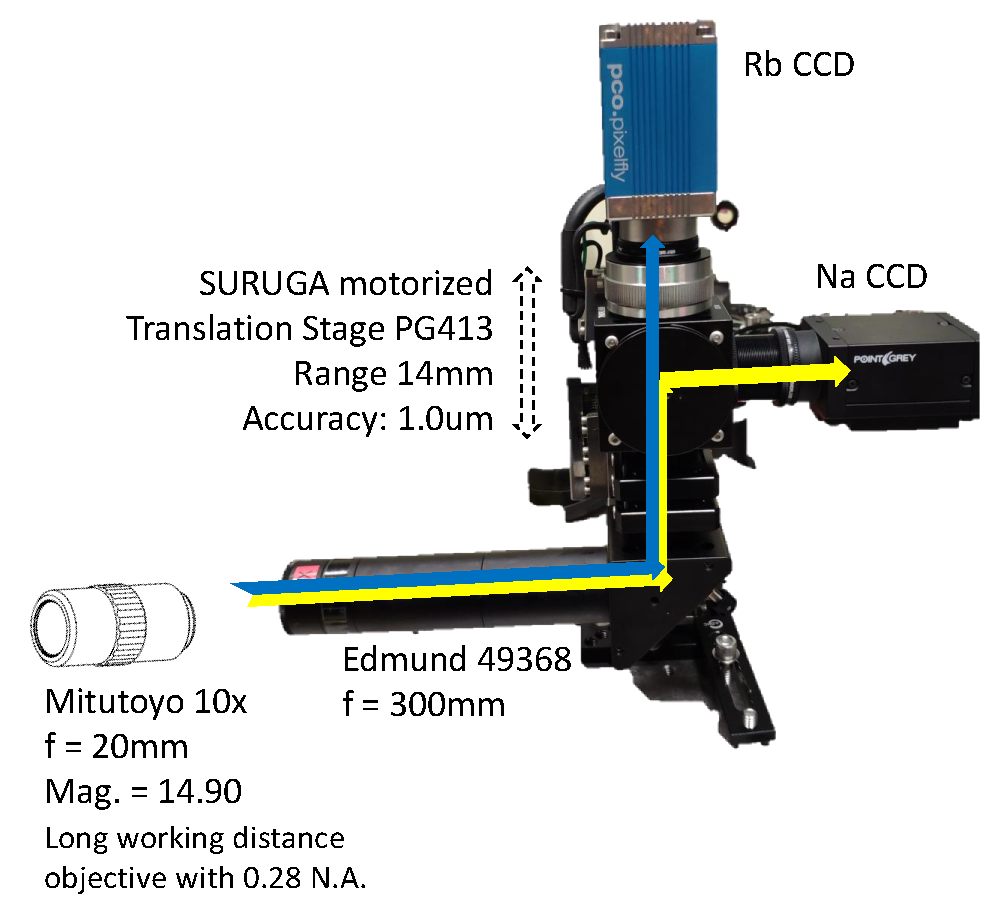
\includegraphics[width = 0.8\linewidth]{figures/image_system.pdf}
\end{center}
\caption{image system}
\label{image_system}
\end{figure}

% coma and translation stage
As we will do TOF for sample for several mm, which could decrease the image resolution. This can be shown be Zemax by a tilted angle of input light. As Shown in Figure.(add) As we use a high magnification iamge system with rather short focus length about 20 mm, this could make its field of view quite small. So, we need to move the whole image system with the movement of atom free-falling. So, we make a compact image system and mount it onto a translation stage controlled by computer. The translation stage is mounted vertically on a 2-axis hand tuned translation stage. Its 型号 is (check), with a resolution 1um (chekc) and repitability 1um(check). We use a arduino board for drive it. finally, we can change the position of our image system at will shot by shot.

\subsection{High magnetic field absorption image}
% aim
To probe the droplet without 失真, we need the probe method reliable which means the method can recover the density profile of the sample as real as possible. Since a typical droplet sample has OD above 50 for Rb and 10(check) for Na, a typical absorption image method cannot be used dirrectly. That is because absoption image's SNR is limited when the sample OD is too high. As plotted in Figure(add), a typical probe intensity can only support OD smaller than 3 (check). With increasing the probe intensity to achiece the saturation absorption image, one can increae the thereshold of OD to probe. However, higher intensity could cause several problems(does high intensity really help for increasing the SNR of sample?) first is calibration could be hard to do or cause large error?(check) second is high intensity image for a high density sample could also induce the effect about high OD which cause non-real of the sample profile. 

% High-field image scheme
\begin{figure}[hb]
\begin{center}
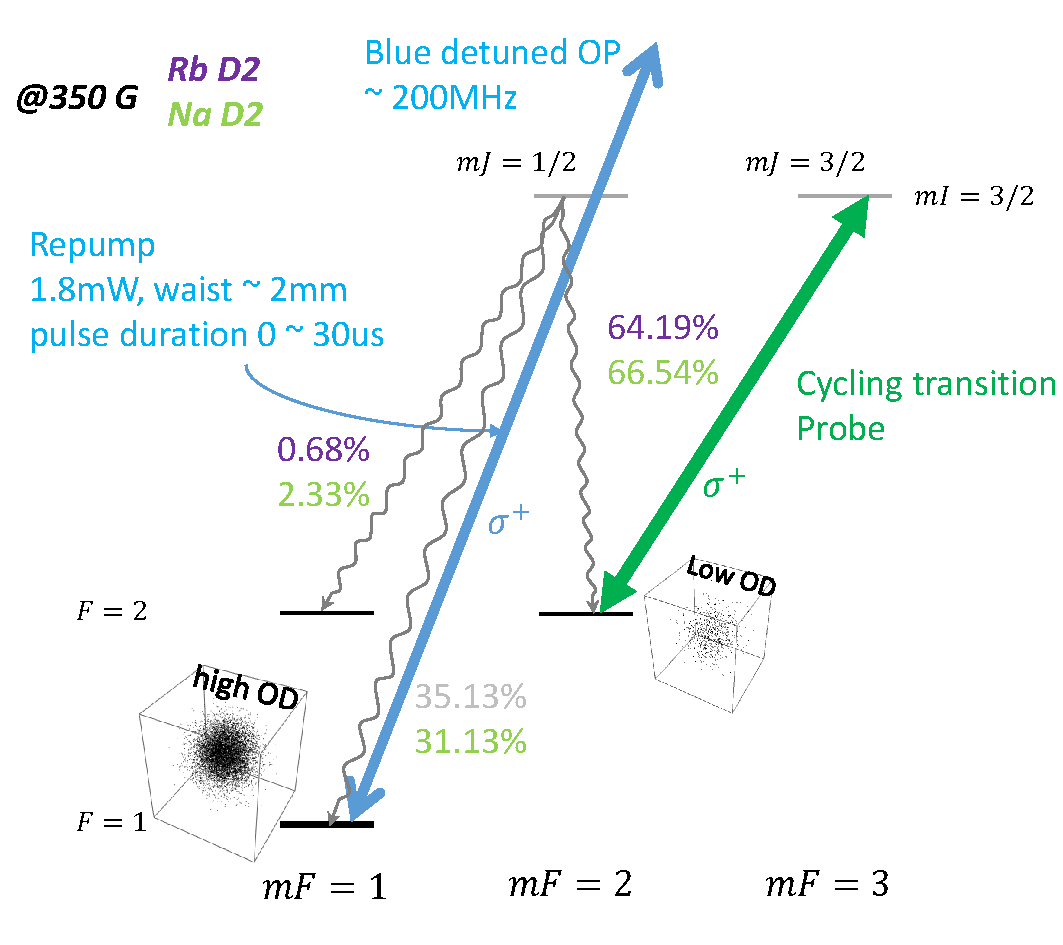
\includegraphics[width = 0.8\linewidth]{figures/High-field image scheme.pdf}
\end{center}
\caption{350 G high field image scheme}
\label{High-field image scheme}
\end{figure}

% How
Thus, a typical method is to first decease the sample's density however keep its profile then do the absorption image, i,e, the partial pumping method for absorption image. A typical way is pumping a small portion of the sample to the image transition by MW or by light. As shown in Figure(add), our sample is 处在 F=1 and mF=1 state which is non reacting with the absortion light. Then, we use a pumping laser to pump the state to p state with F'=2 and F=2 state then with 自发辐射,we accumulate the atom on F=2, mF=2 state and then use the cycling transiton from this state to F=3, mF=3 state to do the absorption image. Here the pumping can also be done by the MW pulse. However a typical MW can only have a Rabi freq less than (check) 10kHz, which could comsume 100us or even longer time to apply a pi pulse. This could make the sample's shape change a lot when we probe it by the image light. So another requirement is to use a shorter pump pulse as better. So, we choose to use the pumping laser, however without using it on resonance, we make it a large detuning and also make it a high intensity. This could make sure even for a very dense sample each layer of the sample could feel around the same intensity which avoid the 不均匀性 of the saturation effect. As plotted in the Figure(add), For xxxx.... (add discription of figure here) (这里描述pupming 光为什么采用这种detuning 和power)Fianlly, we can partial pumping a small portion of the sampel to 2,2 state which can be detected directly. The pumping ratio can be controlled by the duartion of the pumping laser. As shown in the following Figre, a typical pupming fraction as a fuction of duration is ploted. We can see that for the first several tens of us, we have a almost linear puping speed(check) and after 50us(check) we have a saturation effect. This saturation effect is used to calibration latterly. For our experiemtn, to decreae the OD to 个位数sclae, we typical using a detuning 200-300(check)MHz and pumping only several us to achieve a portion less than 10 per cent. Then a typical low intnsity absorption image can afford it.

% partial_pumping
\begin{figure}[hb]
\begin{center}
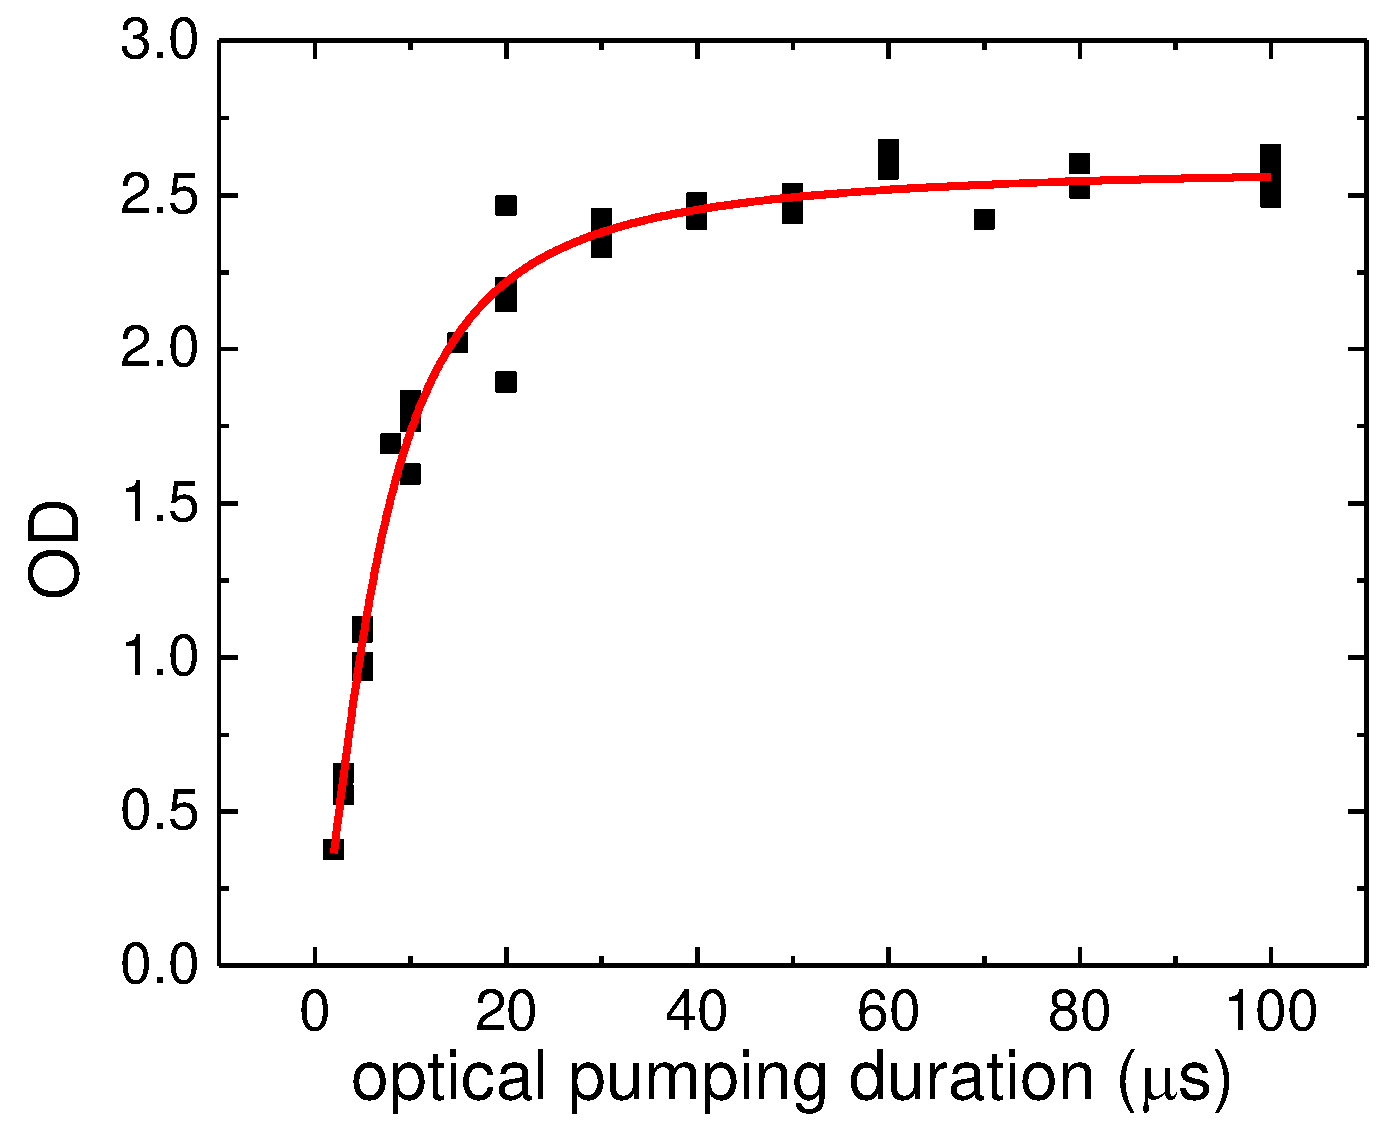
\includegraphics[width = 0.8\linewidth]{figures/partial_pumping.pdf}
\end{center}
\caption{partial pumping}
\label{partial_pumping}
\end{figure}

\subsection{Atomic number calibration}

%aim
As we want to not only measure the size of the sample but also the number of sample to get the critical number of the droplet. So, a reliable recovery of its number is important. This need a carefully calibration of the sample's number. As fomulated (add) the main parameters is the alpha which describe the ratio between effective saturation intensity and the calculated saturated intensity I0, or the ratio betweent he effective cross section and the sigma0. (need restate) 
% not finished

% Image_beta_calibration
\begin{figure}[hb]
\begin{center}
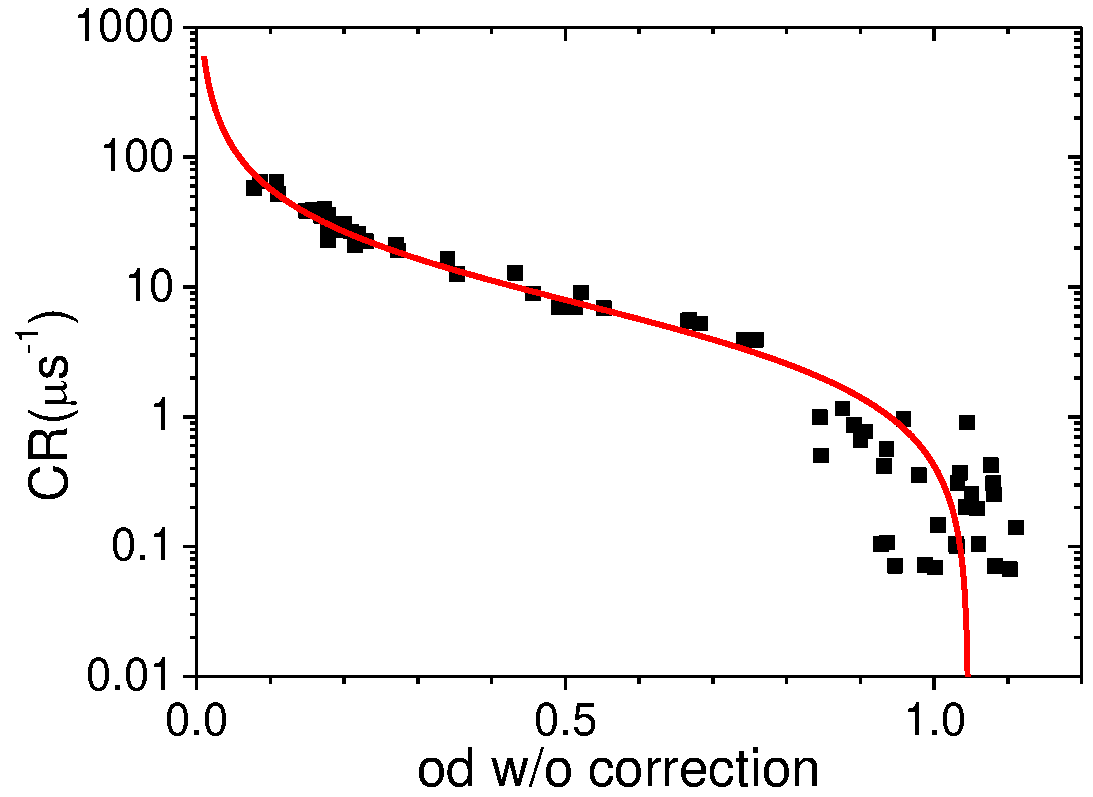
\includegraphics[width = 0.8\linewidth]{figures/Image_beta_calibration.pdf}
\end{center}
\caption{Image_beta_calibration}
\label{Image_beta_calibration}
\end{figure}





\section{Fast magnetic field control}
\subsection{Fast-B coil design and driver}
% why we need fast-B coil
As we mentioned in the section about Feshbach resoannce, by tuning magnetic field we can easily control the scattering properties of atoms, i.e. the interacrion strength. In the precious set-up, we use a large Helmhotz coil with about 90(check) turns. The inductance of the coil is typically 2 mH(need check), which is a very large one with long time contants. (find a better way to describe here). So, even with driver with 100V(check), we will have a rising slope with 1ms(..), which is not fast enough for our requirement to control the interaction. Our request is depend on the time scale of the research object. For example, a typical BEC with as of 100 a0 order will have time scale less than 1 ms. Thus, to control the interaction fast we need about time scale 10 us or even faster. Then we can make sure the sample's size of other paraters changing much slower than the interaction changing.

% What is fast coil and how to build one.
So, with the above request, we need to build another coil which can generate a small but fast magnetic field. The limitation is inductance of the coil, so we reduce its winding to as few as possible. However, with fewer tunes the magnetic field it can generate all declines. So we need make a trade off here. As plotted in the following graph. we can find that their is a best tunes to generate the B-field we want. (Add Figures here) Also, to generate larger magentic field, we put it as close as posible to the cell. Finally, we choose a Helmhots coil with 6 turns in each set. The set-up with Main Feshbach coil is shown here. To adapt our previous large coil. we design a holder made of 聚酰乙烯,查一下是什么。and the holder winding with fast coil is steaked into the 2 inch optical path for MOT beam. 

% current driver and its test data
To driver this fast coil, we need a current driver which can generate fast change of current, so with Lintao's help, we design a fast coil driver with several group of JFET for fast turning on-off and also make a precision control of the current with very few leaking current. The driver schematic can be found in the appendix.C(add here)

% coupling of fast coil and main coil
As shown in JILA's thesis, now, we need to consider the coupling of the fast coil and the main coil and the environment. Since, these coupling will cause oscillation and jiggle when quenching the current in the fast coil. As modeled by the 集总 elements, as shown in figure. (Add figure). The coupling from the main coil and fast coil can be viewed as ... and environment as ... Finally, we have a tested quenching for fast coil.



\subsection{Dynamic compensation for induced and eddy current}
% Why we need dynamic compensation
There are two reasons for us to do the dynamic compensations, first is the coupling of fast coil and main coil and the environment will cause a jigger when we quench the current of the fast coil. To avoid this jigger, we 


\section{Other Technical Issues}
\subsection{Magnetic field gradient compensation}
%Why we need to compensate the B-field gradient 
As mentioned before, we use a pair of Feshbahc coil to generate large bias magntic field to control the Feshbach resonance. However, due to the imperfection of the coil, such as assymetry of each up and down coils and distance not coincident with the Helmhotz coil, the magnetic field typically has a gradient and/or curvature onto the atom. This effect can be easily detect by free-falling of atom in high magnetic field. If one find that the accelaration of the atom is deviated from gravity accelaration, there must be the gradient. Another evidence is the MW (rf) spectroscopy for a elongated sample which could detect the gradient on the horizontal direction. As shown in Figure, we free-fall Rb or Na under high magnetic field, and the accelaration is shown to be differnt from gracity, thus, in our set-up this effect could affect a lot when doing the following experiment with free-falling method. (give more number) 

% What is our gradient looks like?
Before talking about canceling this gradient, we first try to measure it. The method is simple following the MW transition calibration method. We apply the MW pulse coupled the 1,-1 and 2,0 state. Then to get the spacial distribution of the magentic field, we first let the atom free-falling, then apply the MW pulse at differnt TOF. Even though the gradient will affect the position of the atom, considering the samll effect related to g, this can be neglected. Then, we get the magnetid spactial distribution as show in Figure. We can see that there is not only a gradient of the magnetic field but also does the curvature. By a simple quadratic cruve fitting we get the curvature about 1xxx \(G/cm^2\) and an average gradient about xx G/cm. One thing need to be notice here is what we measrued is only the magnetic field gradient on vertical direction, which is the mainly contribution in our case. As we can see in the horizontal direction the accelaration is even much lower than that in veritical direction which infer that this gradient should comes mainly from the wrong distance of the Helmhotz coil.

% How to compensate the grdient and cuvarture
As it is hard to compensate the full of the curvature since to compensate the curvature we need fully recover the helmhotz condition which need much larger magnetic field compare to the several hundred gauss magnetic field. So, to 妥协性质地 solve the question we meet, we degenerate to compensate the avarage gradient to zero inside the interesting TOF we care. So, we can just add a another magnetic gradient on the vertical direction and to change the value of this gradient to find the best compensate point. For the first test, we simply use the half of our up and down shim coil (e.g. up coil). As shown in Figure, we can generate a inversely direction gradient oppposite to the main coil. Then, we simply change the current of the shim coil and test the accelarion of the atom, to find the compensation point. As the dipole moment of Na and Rb is quite different, we can also find the intersect point of them which represents zero average gradient compensation point, as shown in Figure. Finally, we tune the shim coil to the current at the in tersrct and remeasrue the magnetic field with MW spectroscopy method and compare the result with previous non-compensation one as shown in Figure. It is obvious the mean graditn is reduced a lot however the curvature is still there. The compensated gradient and curture is about xxx \(G/cm^2\) and \(xxx G/cm\) now which should be enough for observing BEC mixture free-falling. 


\subsection{Microwave full-wave loop antenna}
% Why we need to build the 2.57GHz and 7.5GHz full-wave loop antenna
As described in Section.xx, the internal states of atom can be controlled by electromagnetic wave. Typically to drive transition between two different hyperfine states, we need use micro-wave(MW) which typical has wavelength about 0.3 m to 3 m, i.e. 300MHz to 300 GHz for frequency in vacuum. For Na and Rb atom, the hyperfine splittings are 1.7 GHz and 6.8 GHz at zero magnetic field. When magnetic field increasing to 350 G (since we typically use the 347 G Feshbach resonance to control the inter-species interaction), the splitting between F=1, mF=1 and F=2, mF=2 states are 2.6 GHz and 7.5 GHz for Na and Rb separately. Thus, we need an antenna which can work well at these frequency. Here, "work well" commonly has two meanings: one is the antenna's standing wave ratio (SWR) is approaching 1, which means it can transmit more power to emitting as EM wave instead of reflecting them back to the power amplifier. Secondly, we need the atom feel the largest amplitude of E-field because the transitions between different F-state is mainly connected be electron dipole, i.e. an electrical dipole transition.(here, need more carefully check) So, the antenna's position, including its distance to atom and its direction angle are both critical to maximum the utility of the antenna. We can define the efficiency fot the above two process as $\mu_trans$ and $\mu_anta$, and the total efficiency is just the multiplication of them.

% talk about near-field and far-field difference
A commercial antenna is typically designed to work well at far field. The radiation power declines inversely proportional to the distance. Thus, in order to increase the power received by atom, we need to put the antenna as close to the atom as possible. However, this renders the radiation felt be the atom turns to be near-field instead of far-field. As depicted in Figure, the electric and magnetic field line (OK?) of a dipole antenna is plotted as blue and red separately. At a large distance of the antenna, the electric field line is almost perpendicular to the \(\hat{r}\) direction. However, when getting closed, it shows more portions to the \(\theta\) direction. This tells us that near-field electromagnetic field of antenna behaves quite different from its far-field one. At far-field region, both electric and magnetic field lines are perpendicular to the Poynting vector, which shows its radiation properties. However, the near-field cannot be treated as a radiation, instead, we typically treat it as "quasi-static" field. A quasi-static field means the distribution of EM field is the same as it in electrostatics, except a oscillation in magnitude with \(e^{i\omega t}\). In engineering, these study is important to wireless-charging, proximity sensors and so on.

% what previous one done, and what's the problem of it
Previously, we use horn antenna for Rb MW transition at 6.8GHz. (add reference here) The distance between horn and atom is about 10-15 cm (check and measure the number). Problem to put the antenna closer to the atom is its huge size which could block the optic path and its metallic body could disturb the strong magnetic field of large Feshbach coil causing a gradient on atom. So the nearest position we can put is about (10 cm) and the measurement Rabi frequency of Rb 1,1 to 2,2 transition at 350 G (7500 GHz) is less than 10kHz (check the number) with a 40 W power amplifier. The correspondents half-\(\pi\) pulse duration is about 50us (check number) which is too long for most of our experiment such as high magentic field image or too weak for dissociating the FR molecule. Thus, we need upgrade it to enhance the Rabi frequency.

% How to improve? what is full-wave loop antenna?
So, a naive solution is try to put the antenna as close to the cell as possible and try to shrink its size smaller and thinner. Therefore, the loop antenna will be a proper choice. A loop antenna is just a simple loop connected to the signal generator. However, for our case with frequency at 2.6 GHz and 7.5 GHz, The wavelength is around several cm to tens of cm. This is comparable to our coil size, which could introduce severe problem on impedance matching. A common solution is making the perimeter of the loop antenna just a full wavelength, which called the full-wave loop antenna. As shown in Figure (add figure), xxxx. when the scale of antenna is closed to wavelength, the distribution of radiation becomes quite different to those samll-loop antenna. This can be explained by a simplified picture, as shown in Figure. at the 接头地方和正对面 current changes with largest amplitude, and there placed two nodes at the quarter wavelength place to the 接头处。However, for small-lopp antenna, the current almost have same phase on the whole coil. Therefore, they have different patterns shown in Figure.

% How the antenna works?
According to the near-field quasi-static EM field theory, we can write down the EM field as following:
\begin{equation}
    E...
\end{equation}
Then, we can plot the radiation power as function of distance to the center of the loop coil, as shown in Figure. The maximum radiation appears at \(\lambda/4\) away from the plane of coil. And actually, the power at the center of coil is zero, which is in opposite to the case of a small-loop coil. For our case with f=2.6GHz, the wavelength is about 12 cm and we place the coil 3 cm away from atom to achieve the largest power. For the 7.5Ghz case, we use paramter about 4 cm coil loop, however we cannot put the coil 1 cm away from the atom since the cell has a size of 2cm, so 综合考虑optical path and power, we put the tiny coil at the side of cell with a 45 degree angle and distance to atom about 3 cm. 

% Set-up and impedance matching
After preparing the coil, we set up the standard MW power amplifier circuit for it. For the 2.6Ghz one, we use (link) from Taobao, and for the 7.5 Ghz one, we use .. from ... Before the amplifier we add a switch controlled by TTL signal and finally the signal generator is SG386. The key point to increase the efficiency from power amplifier to the coil, i.e. \(\eta_{trans}\), we need carefully consider the impedance matching from the transmission wire to eh loop coil. As shown in Figure, we demonstrate several full-wave loop antenna with different shapes. They have different impedance, the ideal one is the rectangular with aspect ratio 1:2, which just have 50 Ohm impedance. However, for our case with round shape, we have the coil with 133 Ohm. our transmission line and power amplifier are all 50 Ohm, so we need to do the impedance matching. Typical we can use a baloon, to simplify we use a 75 Ohm transition line to enhance the transmission rate. As shown in Figure, the signal can be reflected at the boundary of two lines with different impedance, and from 50 ohm to 75 Ohm wire and from 75 ohm to the 133 ohm coil, there exist two reflection wave. If we choose the length of the 75 Ohm line, we can cancel the reflection by superposition two of them. 

% How detail the impedence mathcing works
要配上公式和图片解释这个事情

% Test of the coil
Even though now we know how long the q-section line should be, we still need to do the off-line test for its performance, because a several cm length is to short to allow several uncertainty such as length uncertaainty and 衔接 place different impendence. These imcomplete can cause the phase of replectiong wave shifting and decline the effect of impedence matching. Therefor, we build a series of coil with different length of its q-section, and measrure its return loss rate by a directional coupler. As shown in Figure, we send the siganl into the outpur port of a coupler and the refleting wave from the antenna (connecting on the input port of coupler) will coupled a small portion in to the coupled port and detected by an analyser spectrum. By calculating the reflecting power and injection power, we plot the return loss rate as a function of the length og the q-section line. We can see the period does refer to the half of wavelength and there is a shift which could be attribute the imperfection of q-section line. By fitting with a sine function, we extract the 周期,shift 等等,在列表里。 So, We can now build the coil with lowest return loss for covering our usage frequency.

% Online test
Finally, we put the coil onto the atom cell. First, we test the transmission rate of the coil online to make suere the impedance matching works well, since the offline test with an enviroment open, however the online environment is full of different metals around the coil which could change the boundary condition and shift the impedance of the coil. So, we use the same mathod to test the transmision rate of the coil as shown in Figure. The bandwidth is about xxx MHz. Then, we test the Atomic Rabi frequency to measure the final performance of the coil. We apply the MW pulse for Na at 350 G and get the rabi frequency at different freq or detuning?. As shown in Figure, we test the saturation power and get a Rabi maximum to about 100kHz(check the number). This could allow us to make a pi pulse within 10 us which is enough for most case such as optical pumping in high field and also for MW spectroscopy??.

% about 6.8 7.5Ghz coil
By comfirming the 2.6 GHz coil can work, we turn to use build the 7.5 GHz coil, which could increase the Rabi freq for Rb at high field too. So, we build a similar coil with parameter about 4 cm and its q-section about xx cm, this coil is rather too samll even to put it onto the cell, because it will definitely block some part of the MOT beam. So, finally, we decide to sacrifies some power to put the coil a little bit further away from the coil, i,e, at the corner of the cell, whcih increase the distance of the coild to about 3 cm. Best working distance for the 7.5 Ghz coild should be \(\lambda/4\), i.e. 1 cm, so for 3cm distance we get a power about 1/3 compare to the maximum one (need check number). 总的来说,最后test of the rabi freq is about 100kHz, which recover the previous horn antenna performance. which could allow us to remove the horn antenna (even the coil is working on resonace at 7.5 GHz, when 6.8 Ghz it still can work with a transition rate about \(xxx\%\), so for a typical MW evaporation whichi only consumpted very small power 是足够用的了)

% https://www.everythingrf.com/community/what-is-the-difference-between-a-monopole-and-dipole-antenna
\begin{figure}[htb]
\begin{center}
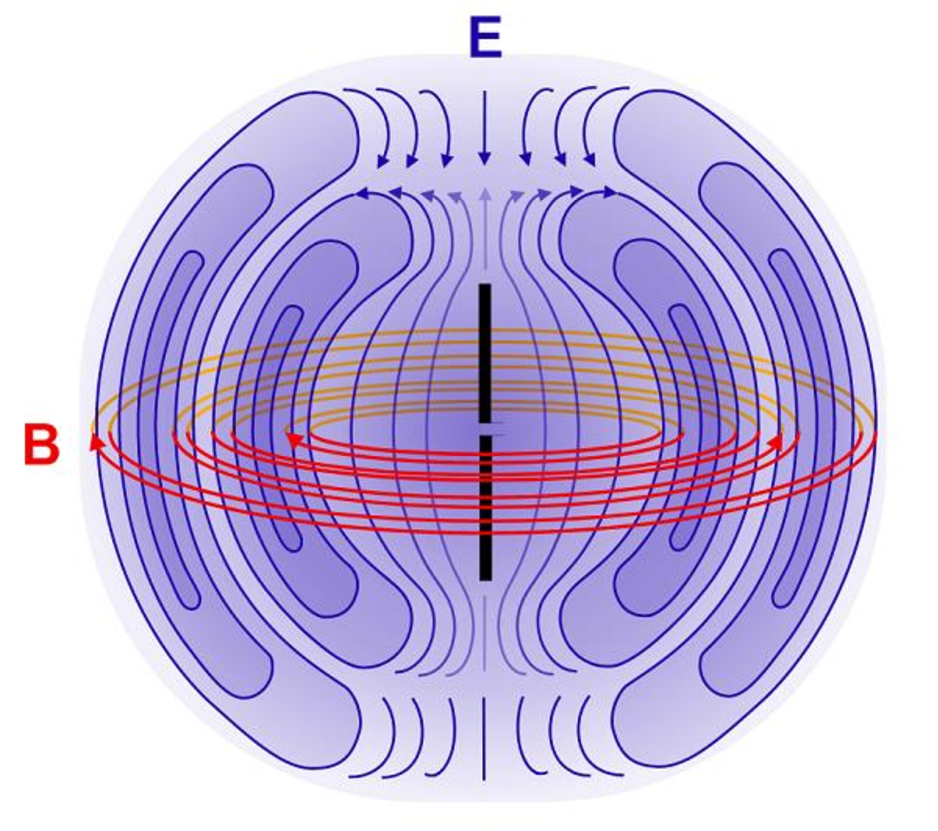
\includegraphics [width =0.5 \linewidth]{Apparatus-EM_field_antenna.pdf}
\end{center}
\caption{}  
\label{antenna_EM}
\end{figure}


\begin{figure}[htb]
\begin{center}
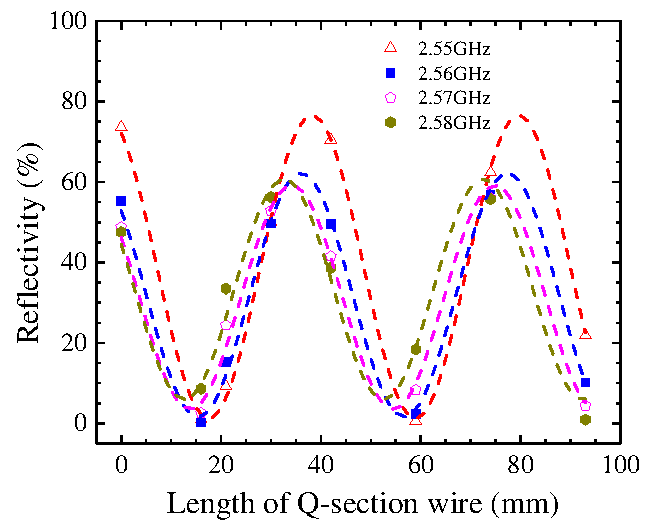
\includegraphics [width =0.7 \linewidth]{Apparatus-loop_antenna_retrun_loss.pdf}
\end{center}
\caption{}  
\label{antenna_return_loss}
\end{figure}

\begin{figure}[htb]
\begin{center}
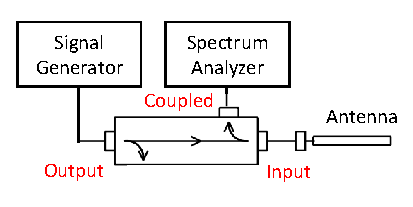
\includegraphics [width =0.7 \linewidth]{Apparatus-measure_SWR.pdf}
\end{center}
\caption{}
\label{SWR_measure_method}
\end{figure}


% How to build the 
